% !TEX encoding = UTF-8
% !TEX TS-program = pdflatex
% !TEX root = ../tesi.tex

%**************************************************************
\chapter{Descrizione dello stage}
\label{cap:Descrizione-dello-stage}

\section{Panoramica del progetto}
L'applicativo in questione è già in attività da circa un anno e ha il compito di pianificare la produzione settimanale degli ordini richiesti dalle varie aziende. Ogni azienda definisce un insieme di linee sulle quali è possibile produrre i prodotti e fornisce anche i giorni e gli orari di lavoro.
\\Con queste informazioni il precedente programma era in grado di fornire una pianificazione distribuita sull'arco della settimana, valutando quale fosse l'ordinamento migliore e quali ordini scartare se il tempo a disposizione non fosse stato sufficiente. Questa logica di pianificazione ometteva però il controllo della disponibilità di materie prime e/o semilavorati,
 la quale veniva considerata sufficiente a produrre tutti gli ordini richiesti.\\ Non veniva inoltre considerato il tempo di produzione degli eventuali semilavorati richiesti, e non si considerava nemmeno l'arrivo di materiali per il magazzino da parte dei fornitori.
Quello che mi è stato richiesto dunque è l'integrazione delle parti sopracitate.

\section{Specifiche tecniche del problema}

Nel primo periodo di stage ho speso il tempo che avevo a disposizione studiando le componenti del problema che dovevo affrontare, ricavando un quadro generale del
 funzionamento logico della pianificazione della produzione. L'ostacolo principale si è rivelato essere la complessità in ambito lavorativo reale della pianificazione.\\
 Ho dovuto spendere del tempo assieme al tutor interno per riuscire ad entrare nel contesto in cui avrei dovuto lavorare, facendomi spiegare le varie sfaccettature e 
 le scelte implementative prese.\\ Di seguito voglio fornire un'idea del problema e di come avviene la pianificazione di un singolo prodotto finito.\\
Perché un prodotto venga pianificato è necessario che ci sia almeno una linea in grado di produrlo, una volta definita la linea si deve scegliere una sequenza in 
cui produrre l'articolo. Una sequenza definisce giorno, data di inizio e di fine e può comprendere un insieme di vincoli da soddisfare
 (quali lavaggi oppure ordinaria manutenzione), l'articolo verrà quindi inserito all'interno della sequenza con il relativo tempo di produzione.
  Ogni linea ha solitamente più sequenze nelle quali è possibile collocare l'articolo. Ogni sequenza può avere dei vincoli di dipendenza con altre sequenze.


\subsection{Implementazione}
Segue la descrizione della struttura delle principali classi che vengono impiegate nell'applicativo.

\subsubsection{Linee}
Indica l'insieme delle linee sulle quali è consentita la produzione degli ordini, ogni linea ha relativo costo orario e definisce l'insieme degli articoli che può produrre con annessa velocità di produzione.
Ogni linea è così definita:
\begin{itemize}
	\item \textbf{Codice Linea}: serve ad indicare su quale linea si vuole produrre l'articolo;
	\item \textbf{Info Articolo}: lista che indica quali articoli la linea può produrre con relativo tempo di produzione;
	\item \textbf{Info Vincolo}: lista che indica i vincoli presenti sulla linea, possono essere obbligatori o opzionali;
	
	\item \textbf{Sequenze Linea}: lista che indica quali sono le sequenze di produzione della linea;
	
	\item \textbf{Pianificazione}: lista che indica quali articoli e quali vincoli sono stati pianificati nella linea corrente;
	
	
	\item \textbf{Errori}: indica quali errori si sono presentati durante la pianificazione;
	
	\item \textbf{Calendario}: indica quali sono i giorni lavorativi con le eventuali pause.
	
\end{itemize}

\subsubsection{Sequenze}
Indica l'insieme delle sequenze di produzione presenti su ogni linea, nelle quali vengono inseriti gli ordini che sono stati pianificati.
Ogni sequenza è così definita:
\begin{itemize}
	\item \textbf{Codice Sequenza}: serve ad indicare su quale sequenza si vuole inserire l'articolo;
	\item \textbf{Giorno}: indica il giorno nel quale si vuole inserire l'articolo;
	\item \textbf{Ora inizio/Ora fine}: indica gli orari di inizio e fine della sequenza corrente;
	
	\item \textbf{Elementi}: lista che indica gli articoli e i vincoli appartenenti alla sequenza corrente.
	
\end{itemize}

\subsubsection{Ordine}
Indica come si presenta un ordine da produrre.
Ogni ordine è così definito:
\begin{itemize}
	\item \textbf{Codice Articolo}: indica il codice dell'articolo;
	\item \textbf{Tipo Articolo}: indica il tipo dell'articolo, può essere un prodotto finito, semilavorato o materia prima;
	\item \textbf{Codice Linea}: indica il livello più generale della gerarchia di classificazione di un prodotto;
	\item \textbf{Codice Settore}: indica il terzo livello di gerarchia di classificazione;
	\item \textbf{Codice Famiglia}: indica il secondo livello di gerarchia, definisce la famiglia del prodotto;
	\item \textbf{Codice SottoFamiglia}: indica il livello più caratterizzante della classificazione di un prodotto;
	
	\item \textbf{Quantità}: indica la quantità richiesta da produrre;
	
	\item \textbf{Data Spedizione}: indica la data di spedizione dell'articolo;
	
	\item \textbf{Ora spedizione}: indica l'ora di spedizione dell'articolo;
	
	\item \textbf{Data Consegna}: indica la data di consegna presso la sede del cliente;
	 
	\item \textbf{Linea preferenziale}: indica la linea preferenziale di produzione dell'articolo;
	
	\item \textbf{Anno Ordine}: indica l'anno dell'ordine in questione; 

    \item \textbf{Materie Prime}: lista che indica l'insieme delle materie prime richieste per la produzione dell'ordine;
  
   \item \textbf{Semilavorati}: lista che indica l'insieme dei semilavorati richiesti per la produzione dell'ordine;
   
   \item \textbf{Riferimento Ordine}: lista che indica l'insieme degli ordini ai quali l'ordine corrente fa riferimento per la produzione di semilavorati;
   
\end{itemize}

\subsection{Problemi logici da affrontare}
Di seguito sono presentate le problematiche che l'algoritmo deve affrontare per ottenere una corretta pianificazione della produzione.

\subsubsection{Temporali}
Qui vengono descritti tutti i problemi riguardanti i tempi di produzione.
\begin{itemize}
	\item \textbf{Data Spedizione}: devono essere rispettate le date di spedizione e di consegna degli articoli da pianificare;
	\item \textbf{Tempo minimo alla consegna}: devono essere rispettate le date di inizio produzione nel caso di ordini con scadenza a breve termine;
	
	\item \textbf{Semilavorati}: i semilavorati di un ordine devono essere pianificati prima dell'ordine stesso;
	
	\item \textbf{Ordini Fornitori}: vanno considerate le date di arrivo delle materie prime da parte dei fornitori in modo da non scartare la produzione di ordini che sarebbero producibili;
	
	\item \textbf{Giorni Lavorativi}: devono essere rispettati i giorni lavorativi senza pianificare ordini al di fuori di essi;
	\item \textbf{Orario Lavorativo}: devono essere rispettati gli orari lavorativi senza eccedere dal monte ore impostato dall'azienda che esegue la pianificazione;
	\item \textbf{Sovrapposizione Sequenze}: ogni linea può produrre una singola sequenza per volta;	
	\item \textbf{Sovrapposizione Articoli}: ogni sequenza può contenere un solo articolo senza sovrapporne degli altri nello stesso lasso di tempo.
\end{itemize}

\subsubsection{Vincoli}
Qui vengono descritti tutti i vincoli da rispettare.
\begin{itemize}
	
	\item \textbf{Materie prime}: non è possibile produrre un ordine se non sono presenti sufficienti materie prime;
	
	\item \textbf{Vincoli Obbligatori}: devono essere pianificati tutti i vincoli obbligatori di ogni sequenza;
	\item \textbf{Vincoli Condizionati}: devono essere pianificati tutti i vincoli condizionati di ogni sequenza in base alle condizioni imposte;
\item \textbf{Vincoli Opzionali}: devono essere pianificati i vincoli opzionali solo in caso ci sia una finestra temporale sufficiente altrimenti si lascia spazio alla produzione di articoli;
	\item \textbf{Vincoli Articolo}: devono essere rispettati i vincoli di produzione di ogni articolo, quali linea preferenziale o linea con maggiore velocità di produzione.
\end{itemize}

\subsubsection{Scelte implementative}
Dopo una discussione col tutor interno abbiamo scartato l'ultimo vincolo facoltativo FA2, presente nel piano di lavoro, il quale riguardava la ripianificazione degli articoli in caso di guasti o necessità aziendali. Optando per una semplice nuova esecuzione dell'applicativo con i nuovi dati interessati. 

\newpage
\section{Obiettivi}

Gli obiettivi da raggiungere durante il progetto sono elencati di seguito, fanno riferimento a quanto riportato nella versione definitiva del piano di lavoro, con qualche aggiunta o modifica in sede di sviluppo, previa discussione con il tutor aziendale.
\\Per ogni obiettivo è definito il grado di completamento: nullo, parziale, totale.

\begin{figure}[h]
	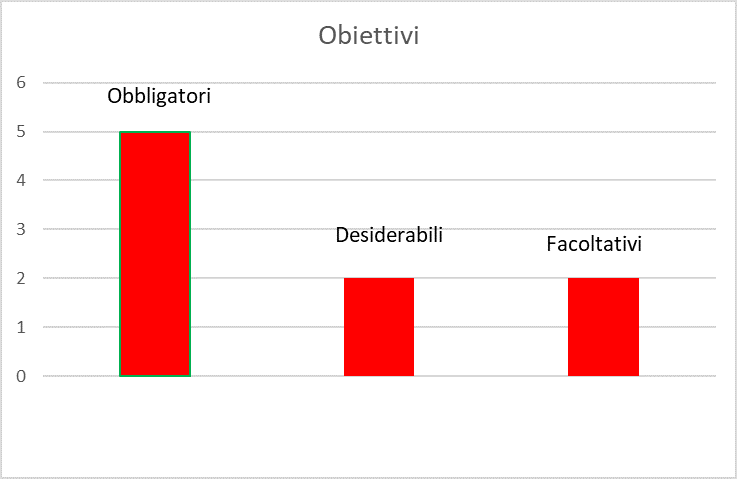
\includegraphics[width=9cm]{immagini/requisiti2.png}
	\centering
	\caption{Requisiti}
\end{figure}


\subsection{Requisiti obbligatori}
\begin{itemize}
	\item Ottimizzazione della pianificazione tenendo conto delle giacenze
	di magazzino: raggiungimento totale;
	\item Sviluppo di nuove strategie di scelta dell’Algoritmo Greedy e
	confronto dei risultati ottenuti in relazione alla funzione obiettivo: raggiungimento totale;
	\item Integrazione della Tabu Search con nuovi criteri di aspirazione e
	arresto: raggiungimento totale;
	\item Sviluppo di nuovi meccanismi di esplorazione del vicinato nella
	Tabu Search: raggiungimento totale;
	\item Acquisizione di competenze sull’utilizzo di algoritmi di Ricerca
	Operativa e applicazione in un caso di studio reale: raggiungimento totale.

	
\end{itemize}

\subsection{Requisiti desiderabili}
\begin{itemize}
	\item Ottimizzazione della pianificazione tenendo conto degli ordini a
	fornitore presenti a sistema: raggiungimento totale;
	\item Ottimizzazione della pianificazione tenendo conto dei
	semilavorati: raggiungimento totale;
\end{itemize}

\subsection{Requisiti opzionali}
\begin{itemize}
	\item Utilizzo di multithreading nelle fasi in cui è richiesta una maggiore
	capacità di calcolo: raggiungimento totale;
	\item Data una pianificazione inserita a sistema, eseguire una
	ripianificazione considerando vincoli dovuti a necessità aziendali
	dell’ultimo momento (anomalie, guasti, ordini urgenti, etc.): raggiungimento nullo.
\end{itemize}

Come accennato nella sezione precedente il requisito FA2 "Data una pianificazione inserita a sistema, eseguire una
ripianificazione considerando vincoli dovuti a necessità aziendali
dell’ultimo momento" è stato scartato a seguito di una riunione con il tutor aziendale. \\Siamo quindi giunti alla conclusione che, in termini di efficacia, è preferibile una nuova esecuzione dell'algoritmo a partire da zero piuttosto che conservare gli attuali dati e procedere con una nuova rielaborazione. Questo rende anche più facile la definizione e l'aggiunta dei nuovi vincoli imposti, quali linee bloccate o sequenze non più attive, che potrebbero influenzare negativamente i precedenti dati inseriti.


\section{Divisione settimanale}

La seguente sezione vuole descrivere come sono state suddivise le 320 ore previste per il periodo di stage, affiancando ad ogni settimana lavorativa i requisiti e gli
 obiettivi raggiunti.\\ Il periodo di stage inizia in data 09-settembre-2019 con termine ufficiale in data 01-novembre-2019 traslata al 03-novembre-2019 a causa del 
 sostenimento di due prove d'esame.

\begin{itemize}
	\item \textbf{Prima settimana}:
	\begin{itemize}
		 \item analisi del modulo software esistente;
		 \item funzionalità da realizzare;
	 	 \item studio della documentazione disponibile dell’algoritmo esistente.
	\end{itemize}
	\item \textbf{Seconda settimana}: 
	\begin{itemize}
		\item analisi dei rischi;
		\item stesura dell'analisi dei requisiti che comprende le nuove funzionalità da integrare nel software esistente;
		\item  inizio della stesura di documentazione a supporto dell'architettura utilizzata.
	\end{itemize}
	\item \textbf{Terza settimana}:
		\begin{itemize}
		\item Studio delle tecnologie aziendali necessarie allo sviluppo del
		modulo in particolare linguaggio di programmazione VB.NET\glo, componenti
		DevExpress\glosp e database Informix\glo;
		\item  training\glosp sulle nuove tecnologie da utilizzare con realizzazione di un software di prova;
		\item studio di algoritmi e tecniche di Ricerca Operativa e	Ottimizzazione Combinatoria;
		\item riunioni col tutor aziendale per decidere le scelte implementative dell'algoritmo Greedy.
	\end{itemize}
	\item \textbf{Quarta settimana}:
		\begin{itemize}
		\item Algoritmo Greedy: sviluppo di nuove strategie di scelta
		del passo successivo adottato dall’algoritmo nella
		costruzione della soluzione del problema;
		\item sviluppo procedura di gestione delle giacenze di
		magazzino.
		\end{itemize}
	\item \textbf{Quinta settimana}:
		\begin{itemize}
		\item sviluppo procedura di gestione dei semilavorati
		pianificati;
			\item sviluppo procedura di gestione degli ordini fornitori.
		\end{itemize}
	\item \textbf{Sesta settimana}:
		\begin{itemize}
		\item integrazione della Tabu Search con nuovi meccanismi:
		criteri di aspirazione e arresto, variazione dei
		meccanismi di esplorazione del vicinato e adozione di
		tecniche di intensificazione e diversificazione.
		\end{itemize}
	\item \textbf{Settima settimana}:
		\begin{itemize}
		\item fase di test dei dati con valori reali forniti dai clienti di Ergon;
		\item comparazione dell'algoritmo ultimato con il precedente algoritmo in uso;
		\item verifica della bontà della soluzione in rapporto coi dati forniti dai clienti.
		\end{itemize}
	\item \textbf{Ottava settimana}:
		\begin{itemize}
		\item stesura della documentazione a supporto del prodotto sviluppato, con risalto sulle scelte implementative non banali.
		\end{itemize}
\end{itemize}

Da sottolineare il fatto che le fasi di test sono state molteplici e non solo durante la settima settimana. Ad ogni nuova aggiunta veniva effettuato un controllo sul risultato prodotto dalla pianificazione con dei dati reali di supporto, tutto ciò per garantire la correttezza della logica del codice in aggiunta. In comune accordo con il tutor abbiamo deciso di iniziare dalle parti più complesse la nuova fase di implementazione, così da garantire una continua verifica ad ogni aggiunta delle funzionalità meno importanti.

\pagebreak
\section{Analisi dei rischi}
Ho trovato importante individuare eventuali rischi che possono portare a problematiche in grado di far procedere a rilento la realizzazione del progetto di stage.\\
Di seguito viene presentata la tabella contenente i rischi preventivati durante la seconda settimana di stage. Ogni rischio possiede un codice identificativo, una breve descrizione affiancata dal suo rilevamento e relativo grado di rischio. Per ogni rischio è definito inoltre un piano di contingenza da seguire in caso di occorrenza del rischio.



\renewcommand{\arraystretch}{1.5}
\rowcolors{2}{dispari}{pari}
\arrayrulecolor{white}
\begin{longtable}{ 
		>{\centering}p{0.17\textwidth} 
		>{\raggedright}p{0.28\textwidth}
		>{\raggedright}p{0.29\textwidth} 
		>{\centering}p{0.15\textwidth}
	}
	
	\caption{Tabella dei rischi di progetto}\\
	\rowcolorhead
	\colorhead\textbf{Codice \\ Nome} & \centering\colorhead\textbf{Descrizione} & 
	\centering\colorhead\textbf{Piano di contingenza} & 
	\colorhead\textbf{Grado di rischio} 
	\tabularnewline
	\endfirsthead
	\rowcolor{white}\caption[]{(continua)}\\
	\rowcolorhead
	\colorhead\textbf{Nome \\ Codice} & \centering\colorhead\textbf{Descrizione} & 
	\centering\colorhead\textbf{Rilevamento} & 
	\colorhead\textbf{Grado di rischio} 
	\tabularnewline
	\endhead
	
	%RO1---------------------------------------------------------
	\rowcolordark \textbf{RO1} \\ Problematiche di Ricerca Operativa & 
	Dovendo svolgere uno studio individuale delle tematiche di Ricerca Operativa da affrontare, è possibile imbattersi in argomenti poco intuitivi o complicati da apprendere in solitaria. &
	Vengono fornite le dispense riguardanti il contesto in cui si andrà a lavorare e in caso di incomprensioni si farà affidamento sia sul tutor interno sia al proprio relatore. &
	Occorrenza: \textbf{Media} \\
	Pericolosità: \textbf{Alta} 
	\tabularnewline
	
	%RT1---------------------------------------------------------
	\rowcolorlight \textbf{RT1} \\ Inesperienza tecnologica & 
	Alcune delle tecnologie adottate sono nuove, pertanto è possibile incorrere in problemi durante lo svolgimento delle attività che le coinvolgono. &
	Viene fornita la documentazione ufficiale in modo da avere ampio supporto per qualsiasi lacuna di natura tecnica. Se ciò non dovesse bastare si farà affidamento al tutor interno o qualche membro delegato del team di sviluppo di Ergon. &
	Occorrenza: \textbf{Media} \\
	Pericolosità: \textbf{Media} 
	\tabularnewline

	%RT2---------------------------------------------------------
	\rowcolordark \textbf{RT2} \\ Scelte implementative & 
	Non è detto che tutte le scelte prese in considerazione durante lo studio del problema portino ad una corretta soluzione o ad una esecuzione in tempi accettabili. &
	Verranno valutate, in caso di necessità, nuove strade da percorrere per la risoluzione del problema. &
	Occorrenza: \textbf{Bassa} \\
	Pericolosità: \textbf{Alta} 
	\tabularnewline
	
	
\end{longtable}
	
\renewcommand{\arraystretch}{1}